\documentclass[11pt]{article}

% "review" for submission (anonymous, line numbers); "final" for camera-ready; "preprint" for arXiv.
\usepackage[review]{acl}
% lineno v5.7 (2026/02) writes its column tag from the build/column/before hook, one column late, which misplaces
% right-column line numbers in two-column review mode. Tag the finished column box instead.
\makeatletter
\ifdefined\RemoveFromHook
  \RemoveFromHook{build/column/before}[lineno]
  \AddToHook{build/column/after}{\setbox\@outputbox\vbox{\boxmaxdepth\@maxdepth
    \protected@write\@auxout{}{\string\def\string\@LN@column{\if@firstcolumn1\else2\fi}}\box\@outputbox}}
\fi
\makeatother

\usepackage{times}
\usepackage{latexsym}
\usepackage[T1]{fontenc}
\usepackage[utf8]{inputenc}
\usepackage{microtype}
\usepackage{inconsolata}
\usepackage{graphicx}
\usepackage{booktabs}
\usepackage{amsmath}
\usepackage{xcolor}
\usepackage[most]{tcolorbox}
\usepackage{pifont}

% Drafting marks: remove before submission.
\newcommand{\todo}[1]{\textcolor{red}{[TODO: #1]}}

% Boxed takeaways (one per main results section), as in Wang et al. (2026).
\newcounter{takeaway}
\newtcolorbox{takeaway}{enhanced, breakable, colback=gray!5, colframe=gray!60, boxrule=0.5pt, arc=1.5pt,
  left=5pt, right=5pt, top=3pt, bottom=3pt, fontupper=\small,
  title={\stepcounter{takeaway}\textbf{Takeaway \thetakeaway}}, fonttitle=\small, coltitle=black,
  colbacktitle=gray!15, attach title to upper={\ }}

\title{Judges Approve What They Believe:\\An LLM Judge's Own Answers Predict Which Wrong Answers It Accepts}

\author{Anonymous ACL submission}

\begin{document}
\maketitle

% ---------------------------------------------------------------------------------------------------------------
\begin{abstract}
Recent work ties LLM judges' approval of wrong answers to whether the judge can answer the question itself. We test
this per answer: the judge's \emph{belief} in a candidate written by another model is the share of its seven
independent answers that reach the candidate's final answer. Across three benchmarks and seven judges from four
families, approval of wrong answers rises with belief, from 1--25\% when the judge never reaches the answer to
47--86\% when it always does (two judges rise less). Pooled across judges, the association persists after
controlling for question identity and under a second auditor's labels, and seven samples predict approval better
than one. Under protocols fixed before data collection, it replicates on 1,336 fresh multiple-choice pairs (19\% at
0/7 to 63\% at 7/7) and, more weakly, on 819 open-ended math pairs with exact integer matching (4\% to 92\%, but all 13
judgments at 7/7 are on disputed keys, and the same-candidate test is null). Model auditors dispute benchmark labels
more often for the answers judges believe most (multiple choice 9\% vs 51\%; math 2\% vs 7 of 7). Explanations and
hidden states are consistent with the result but do not identify a mechanism.
\end{abstract}

% ---------------------------------------------------------------------------------------------------------------
\section{Introduction}

LLM-as-a-judge is now a standard way to score open-ended outputs, build preference data and run benchmarks
\citep{zheng2023judging}. Its best-known failure is self-preference: judges rate their own generations higher
\citep{panickssery2024llm}. Two recent results point to a different reading. Much of what looks like
self-preference can be explained by the judge being wrong about the question \citep{roytburg2026narcissists}, and
judges agree with human experts mainly on questions they can answer themselves \citep{krumdick2026nofreelabels}.
Both suggest that what matters is the judge's own \emph{answer} to the question, not who wrote the text it grades.
Both, however, measure this per question or per model, so they cannot say which of a judge's errors it will make.

We therefore measure it per answer (Figure~\ref{fig:overview}). Every judge grades answers written by other models,
so self-authorship is excluded by design (style shared within a model family remains possible). Separately, and
without seeing any candidate, the judge answers the same question seven times. Its \emph{belief} in a candidate is
the share of those answers that reach the candidate's final answer, from 0/7 to 7/7. We ask whether belief predicts
which wrong answers a judge approves, whether alternative explanations account for it, and whether it replicates
on questions we had not analysed.

This is not self-preference under another name. Self-preference concerns who wrote the text: judges favour their own
generations, and the bias tracks how familiar (low-perplexity) a text is to the judge
\citep{panickssery2024llm,wataoka2024self}. Belief concerns what an answer concludes. Our judges never grade their
own text, and, pooled across judges, the association holds in two narrower comparisons: among wrong answers
to the same question graded by the same judge (difficulty fixed), and for the same candidate graded by judges that
believe it to different degrees (author fixed, though how close each judge's family is to the author's can still
differ; \S\ref{sec:staircase}). A believed conclusion may also read as more familiar to the judge;
we count that as part of what belief measures, not as a separate explanation.

\begin{figure*}[t]
\centering
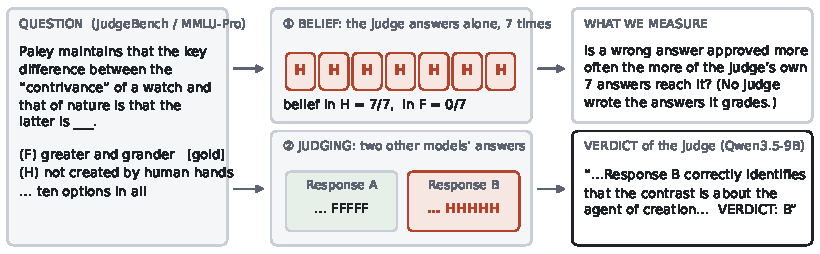
\includegraphics[width=\textwidth]{figures/overview.pdf}
\caption{How belief is measured, on a real JudgeBench item. \ding{172}~Without seeing any candidate, the judge
answers the question seven times; its belief in an answer is the share of these that reach it. \ding{173}~The judge
then grades answers written by other models. Here Qwen3.5-9B reaches the wrong option~H in all seven tries and,
shown two responses, picks the one that answers~H. Both label auditors (\S\ref{sec:setup}) agree that H is wrong.}
\label{fig:overview}
\end{figure*}

Approval of wrong answers rises with belief in all four families, though two judges (Nemotron-3-Nano and Qwen3.5-4B) rise less
(\S\ref{sec:staircase}). The association persists within question, under alternative labels and, for the Qwen judges, with thinking enabled, and seven samples predict approval better than one. It replicates on fresh multiple-choice questions, and in weaker form on open-ended math
questions, under protocols fixed in advance, with sensitivity analyses for answer parsing and labels (\S\ref{sec:replication}). Written
explanations and hidden states are consistent with the behavioural result but do not identify a mechanism
(\S\ref{sec:process}). Finally, we test three fixes suggested by the result (\S\ref{sec:juries}).

\paragraph{Contributions.}
\begin{itemize}
\item A per-answer measure of judge belief, and evidence from seven judges in four families that approval of wrong
answers rises with it, with controls for question identity, a single matching sample, label noise and reasoning.
\item Two replications with protocols fixed before data collection, on 1,336 new multiple-choice pairs and on 819
open-ended math pairs compared by exact integer match, each with a complete label audit.
\item A label audit in which model auditors dispute benchmark labels most often for the answers judges believe
most, and a cautionary result on reading belief from hidden-state directions.
\end{itemize}

% ---------------------------------------------------------------------------------------------------------------
\section{Related Work}

\paragraph{Judges and their own answers.}
\citet{panickssery2024llm} show that judges recognise and prefer their own generations.
\citet{roytburg2026narcissists} argue that much of this preference reflects the judge being wrong on the question;
we measure that belief per answer and exclude self-authorship. \citet{krumdick2026nofreelabels} find that judges
agree with experts mainly on questions they can answer, and that expert references help; we use their BFF-Bench data
and measure belief per answer on a 0--7 scale. \citet{goel2025great} show that judges favour models that make the same
mistakes; ours is a per-answer version of this model-level effect. \citet{lin-etal-2025-before} find that solving and
judging ability are only weakly correlated, and that giving the judge its own answer as a reference strengthens the
link. \citet{verga2024replacing} propose juries of diverse models to reduce individual judges' biases. We test these remedies and a reference answer by belief level (\S\ref{sec:juries}).

\paragraph{Truth and belief inside models.}
Linear directions separate true from false statements in hidden states \citep{marks2024geometry,burns2023discovering,
azaria-mitchell-2023-internal}, and difference-of-means directions can steer behaviour
\citep{rimsky-etal-2024-steering,arditi2024refusal,zou2023representation}. Whether such probes read truth or the
model's belief is debated \citep{herrmann2025standards}: a ``correctness'' probe can behave like the model's belief
\citep{yang2026admit}, output confidence tracks belief rather than truth \citep{cho2026confidence}, and for judges,
correctness labels alone cannot separate truth from the judge's belief \citep{gulati2026auditing}.
\citet{mukherjee2026opening} find that judges' activations often hold the right preference when the verdict is
wrong. We compare believed and unbelieved wrong answers to the same question, which controls for what a question
looks like to the model.

% ---------------------------------------------------------------------------------------------------------------
\section{Experimental Setup}
\label{sec:setup}

\paragraph{Benchmarks.}
Every item is a question, a candidate answer written by another model, and a right/wrong label.
\textbf{RewardBench~2 Math} \citep{malik2025rewardbench2}: 732 single answers to 183 questions with short final
values. \textbf{JudgeBench} \citep{tan2025judgebench}: 547 response pairs for 459 multiple-choice questions (coding
pairs dropped); the judge picks the better response, and ``approving'' the wrong response means picking it.
\textbf{BFF-Bench} \citep{krumdick2026nofreelabels}: 459 answers to 298 finance questions with unanimous expert labels,
single- and two-turn. \textbf{BBEH} \citep{kazemi-etal-2025-big}: about 2,000 answers to hard reasoning puzzles,
used only for the hidden-state analysis. We chose benchmarks with short checkable final answers, so that a judge's
own answers can be compared with a candidate's.

\paragraph{Judges.}
Qwen3.5-4B, Qwen3.5-9B and Qwen3.6-35B-A3B (Alibaba); Nemotron-3-Super-120B-A12B and Nemotron-3-Nano-30B-A3B
(NVIDIA); DeepSeek-V4.1-Flash (DeepSeek); and Kimi-K2.6 (Moonshot), so that the result does not rest on one
developer's training. Verdicts were collected through a hosted API (Tinker). Nemotron-3-Nano's verdicts come from an
earlier run; by the time we measured belief the API no longer served it, so its own answers were generated on our
GPUs with vLLM, using the same prompts and sampling settings. Each judge writes a short justification and ends with
a verdict line; reasoning (``thinking'') is off unless stated. No judge wrote any of the candidates it grades,
although some candidates may come from other models of the same family. Approval is the verdict the judge
states.\footnote{Reading the verdict instead from the probabilities of the two verdict words at the end of the
judge's own transcript gives the same label on 97--100\% of judgments per family.}

\paragraph{Belief.}
Because a judge's answer to the same question varies from sample to sample, we measure how often it reaches each
answer rather than whether one sample does. For each question the judge answers seven more times at temperature 0.7,
with only the question (and, for two-turn BFF-Bench items, the earlier turns) in context. Belief in a candidate is the number of these answers that reach the
candidate's final answer, divided by the number of valid comparisons (at least five). The endpoint labels 0/7 and
7/7 denote no matches and all matches among the sampled answers; they do not imply underlying answer probabilities
of zero or one. Bins are formed by rounding seven times belief (98\% of audited wrong-answer judgments have all seven
comparisons). Belief is thus an operational answer-frequency measure at one sampling configuration (seven samples,
temperature 0.7, thinking off). A separate, eighth answer defines the one-sample ``matches my answer'' label, the
natural single-answer version of ``the judge can answer''. JudgeBench letters are matched exactly when both answers state one.
Otherwise, and on RewardBench~2 Math and BFF-Bench, GLM-5.3-Flash decides whether two final answers are the same, ignoring wording and rounding
(Appendix~\ref{app:matcher}); a second model reader (Claude) agreed with 42 of 47 of its decisions.

\paragraph{Label audit.}
A ``wrong'' answer that a judge reaches in all seven tries is either a confident error or a label error, so before
analysing approvals we audited every wrong-labelled answer for which the benchmark provides a reference (1,091 unique answers; 13 wrong-answer judgments lack one). GLM-5.3 (high reasoning) read each with the
question and the benchmark's reference, was told the reference may itself be wrong, and labelled the answer
\emph{clearly wrong}, \emph{actually correct} or \emph{contested} (Appendix~\ref{app:audit}). Kimi-K3.1-Pro, an
auditor from another model family (and from the same developer as the Kimi-K2.6 judge), repeated the audit; the two
make the same clearly-wrong-or-not call on 96\% of answers (Cohen's $\kappa$, agreement beyond chance, 0.77). Claude Opus 5.5 audited 98 answers as a
third check (Appendix~\ref{app:audit}). Audit verdicts are model classifications, not human-adjudicated ground
truth, and auditors can share errors. Unless stated otherwise, results keep only wrong answers GLM-5.3 calls clearly
wrong.

\paragraph{Statistics.}
Intervals are 95\% bootstrap intervals that resample whole questions (2,000 draws). Effects of belief are slopes
from a linear probability model (a linear regression of the 0/1 verdict) with benchmark-by-judge fixed effects (a
separate intercept for each judge on each benchmark), reported as the change from belief 0/7 to 7/7 in
percentage points.

% ---------------------------------------------------------------------------------------------------------------
\section{Approval Rises with Belief}
\label{sec:staircase}

\begin{figure*}[t]
\centering
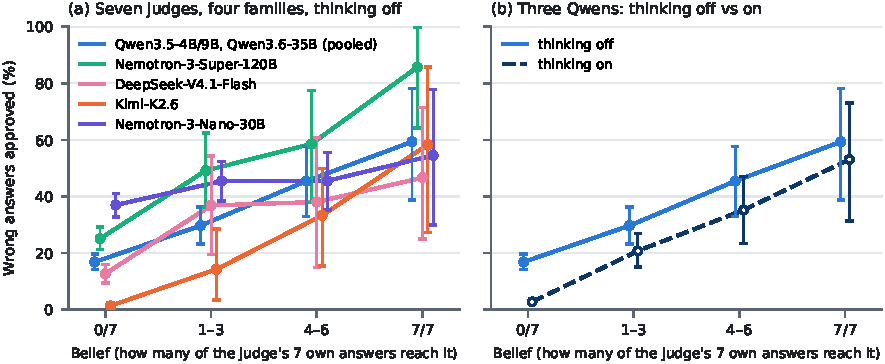
\includegraphics[width=\textwidth]{figures/staircase.pdf}
\caption{Wrong answers approved, by the judge's belief in them (RewardBench~2 Math, JudgeBench and BFF-Bench;
audited labels). (a) Seven judges from four families, thinking off. (b) The three Qwen judges on the same answers with thinking
off and on. Whiskers: 95\% intervals resampling questions.}
\label{fig:staircase}
\end{figure*}

\paragraph{Main result.}
If what matters is whether the judge would give the answer itself
\citep{roytburg2026narcissists,krumdick2026nofreelabels}, a judge should approve the wrong answers it reaches more
often than those it does not. We pool the three benchmarks and group each judge's wrong answers by belief: never
reached (0/7), sometimes (1--3), mostly (4--6) and always (7/7). Figure~\ref{fig:staircase}a and
Table~\ref{tab:families} show that wrong answers the judge never reaches are approved 1--25\% of the time by the
pooled Qwens, Nemotron-3-Super, DeepSeek and Kimi, and wrong answers it always reaches 47--86\% of the time, with
gap intervals excluding zero. Nemotron-3-Nano approves 37\% of wrong answers it never reaches and rises less (+18
[$-$11, +43]; linear slope +17 [+2, +31]). The 7/7 groups are small after the audit (10--15 judgments per judge),
so the top of each curve is imprecise; individually, all three Qwens point the same way, but Qwen3.5-4B's interval
includes zero (Appendix~\ref{app:robust}).

\begin{table}[t]
\centering
\small
\setlength{\tabcolsep}{4pt}
\resizebox{\columnwidth}{!}{%
\begin{tabular}{lrrrrr}
\toprule
Judge & 0/7 & 1--3 & 4--6 & 7/7 & Gap \\
\midrule
3 Qwens (pooled) & 17 & 30 & 45 & 59 & +43 {\scriptsize[+20, +62]} \\
Nemotron-3-Super & 25 & 49 & 59 & 86 & +61 {\scriptsize[+40, +77]} \\
DeepSeek-V4.1-Flash & 13 & 37 & 38 & 47 & +34 {\scriptsize[+9, +58]} \\
Kimi-K2.6 & 1 & 14 & 33 & 58 & +57 {\scriptsize[+23, +87]} \\
Nemotron-3-Nano & 37 & 45 & 46 & 55 & +18 {\scriptsize[$-$11, +43]} \\
\midrule
\multicolumn{6}{l}{\emph{As released (no audit)}} \\
3 Qwens (pooled) & 18 & 35 & 54 & 74 & +56 {\scriptsize[+44, +66]} \\
\bottomrule
\end{tabular}}
\caption{Wrong answers approved (\%), by belief, audited labels. Gap: 7/7 minus 0/7 in points. Group sizes at 7/7:
32, 14, 15, 12 and 11 judgments.}
\label{tab:families}
\end{table}

\paragraph{One sample or seven?}
Because a judge's answers vary across samples, a single sampled answer is a noisy estimate of what it would answer,
so belief might simply be a less noisy version of the one-sample label. Fitting both together (judge fixed effects),
the Qwens' approval rises by +43 points [+26, +57] with belief while the one-sample label adds +2 [$-$9, +12]; the other families agree (Appendix~\ref{app:robust}, Table~\ref{tab:robust}). Since seven samples cost seven times one, we also asked how much
each sample buys, predicting approval on held-out questions with $k$ of the seven samples (Appendix~\ref{app:budget}, Table~\ref{tab:budget}).
Held-out Brier score (mean squared error of the predicted approval probability) falls at each tested $k$: 0.1595 with judge-by-benchmark intercepts only, 0.1572 with one sample,
0.1556 with three and 0.1549 with seven (seven vs one: $-$0.0022 [$-$0.0037, $-$0.0010]). The gains are small in
absolute terms (AUROC, the chance that a random approval is scored above a random rejection, 0.70 to 0.73): belief shifts approval rates substantially but leaves most individual verdicts
unpredictable. The separate eighth answer does not detectably improve on the intercepts here, but it was generated
in an earlier run with a shorter token budget, so it is not exchangeable with the seven; in the MMLU-Pro replication, where it is, it keeps a small association that is sensitive to label filtering, and on
math it is not detectable (\S\ref{sec:replication}).

\paragraph{Re-measuring belief.}
Belief is estimated from seven samples, so we tested its reliability: six of the original judges (Nemotron-3-Nano is
no longer served) answered every original JudgeBench question seven more times. On the 237 audited wrong-answer
judgments in which the candidate and at least five new answers state a letter, new and original belief correlate at 0.87 and agree on the bin 69\% of the
time, and the original approvals rise with the new belief as much as with the original (+50 [+32, +66] vs +48 [+30,
+65]).

\paragraph{Question difficulty.}
On hard questions a judge's answers scatter onto wrong values, and judges might simply be more lenient on hard
questions, which would produce the same pattern. Belief, however, belongs to a (judge, answer) pair, while
difficulty belongs to a question. Comparing only wrong answers to the \emph{same} question graded by the \emph{same}
judge (judge$\times$question fixed effects; 169 such groups, from 88 questions, have answers at different belief
values), the answer believed more is approved more: +47 points [+27, +70]. This pooled estimate is not uniform: it
is clear for the Qwens, Nemotron-3-Super and Nemotron-3-Nano, uncertain for DeepSeek (+45 [$-$9, +86]) and absent
for Kimi-K2.6 ($-$13 [$-$69, +24]; 11 groups). Leaving out any one family keeps it between +41 and +54 with
intervals above zero (Appendix~\ref{app:robust}). Controlling instead for the judge's accuracy on the question, the
belief effect is +49 [+16, +72] while accuracy adds +1 [$-$7, +8], although for individual judges accuracy can
matter as well (Nemotron-3-Nano +15 [+0, +30], Kimi-K2.6 $-$13 [$-$23, $-$3]).

\paragraph{The same candidate across judges.}
Some wrong answers may be persuasive to every model, and models share mistakes \citep{goel2025great}, so a belief
held by every judge could be a property of the answer rather than of the judge. Holding the candidate fixed and
comparing judges that believe it to different degrees (candidate and benchmark-by-judge fixed effects; 313
candidates across 251 questions), the judge that believes it more approves it more: +20 points [+9, +31]. Adding
judge-by-question fixed effects leaves +21 [$-$6, +47], which is inconclusive. Neither specification randomizes
belief.

\paragraph{Alternative labels.}
Because a believed wrong answer may be right, we compared released and audited labels. Without the audit the
Qwens' gap is larger (+56 [+44, +66]; Table~\ref{tab:families}): among the BFF-Bench and JudgeBench answers some Qwen
reaches 7/7, GLM-5.3 calls 23 clearly wrong and 23 actually correct, against 169 and 1 at 0/7 (Table~\ref{tab:audit}),
and judges approve the answers it calls actually correct 61--81\% of the time. The gap remains under the second
auditor's labels and under labels both auditors agree on (Qwens +38 [+20, +56] and +35 [+13, +57];
Appendix~\ref{app:robust}), except for Kimi-K2.6 under both auditors (5 judgments at 7/7) and Nemotron-3-Nano.

\begin{table}[t]
\centering
\small
\setlength{\tabcolsep}{4pt}
\begin{tabular}{lrrrr}
\toprule
Highest & Clearly & Actually & Con- & Approved if \\
belief & wrong & correct & tested & act.\ correct \\
\midrule
0/7 & 169 & 1 & 4 & 4/5 \\
1--3 & 89 & 5 & 6 & 63\% (19) \\
4--6 & 41 & 10 & 14 & 61\% (28) \\
7/7 & 23 & 23 & 9 & 81\% (47) \\
\bottomrule
\end{tabular}
\caption{GLM-5.3 audit of the wrong-labelled BFF-Bench and JudgeBench answers in the Qwen judges' data (unique
answers, binned by the highest belief any Qwen judge has in them; 5 without a verdict). Last column: share of
judgments approving answers the auditor calls actually correct (number of judgments).}
\label{tab:audit}
\end{table}

\paragraph{Thinking.}
If approvals of believed wrong answers came from not checking the candidate, letting the judge reason before its
verdict should remove them. The three Qwens also judged every answer with thinking enabled (belief still measured
with thinking off). On the same audited answers (Figure~\ref{fig:staircase}b), approval rises from 3\% at 0/7 to
53\% at 7/7 (gap +50 [+28, +71], against +43 with thinking off): thinking makes judges stricter on answers they do
not believe (17\% $\rightarrow$ 3\% at 0/7) with no detectable change in the gap (+8 [$-$9, +26]).

\begin{takeaway}
In each of four model families, a judge approves a wrong answer more often the more of its own independent answers
reach it (1--25\% at 0/7 to 47--86\% at 7/7). Pooled across judges, the association persists after controlling for
question identity (not for Kimi-K2.6), under a second auditor's labels and, for the Qwens, with thinking on, and seven samples predict approval better
than one; the most
restrictive same-candidate specification is inconclusive.
\end{takeaway}

% ---------------------------------------------------------------------------------------------------------------
\section{Two Replications on Fresh Questions}
\label{sec:replication}

\paragraph{Multiple-choice setup.}
The analyses above were developed on the same data they are reported on, and flexible analysis choices can produce
spurious findings \citep{simmons2011false}. The benchmarks have no unused questions, so we rebuilt JudgeBench's
construction on new ones, twice: on multiple-choice questions and on open-ended math. For each, the protocol, analyses
and sample size were fixed in writing before collecting data (Appendix~\ref{app:replication}); the protocols are
released with the code but were not registered with a third party. From MMLU-Pro questions JudgeBench does not contain, Nemotron-3.5-Super (NVIDIA)
wrote six answers each; the 1,336 of 6,000 questions with at least one right and one wrong answer became pairs (one
right, one wrong response, random order). Four judges from three families other than the writer's (Qwen3.6-35B-A3B,
Qwen3.5-9B, DeepSeek-V4.1-Flash, Kimi-K2.6) picked the better response and answered each question eight times with
the original prompts; the first answer gives the one-sample label and the other seven give belief. Labels are
MMLU-Pro's answer key.

\begin{table*}[t]
\centering
\small
\setlength{\tabcolsep}{4pt}
\resizebox{\textwidth}{!}{%
\begin{tabular}{lllrrrrrrrr}
\toprule
Judge & Parser & Labels & Judgments & 0/7 & 1--3 & 4--6 & 7/7 & Slope & Same candidate & One-sample label \\
\midrule
\multicolumn{11}{l}{\emph{Per judge, answer key}} \\
Qwen3.6-35B-A3B & strict & key & 742 & 15 & 39 & 56 & 74 & +61 {\scriptsize[+50, +71]} & & \\
 & lenient & key & 1,318 & 13 & 35 & 52 & 72 & +59 {\scriptsize[+51, +67]} & & \\
Qwen3.5-9B & strict & key & 960 & 21 & 42 & 45 & 53 & +34 {\scriptsize[+25, +44]} & & \\
 & lenient & key & 1,327 & 22 & 42 & 48 & 54 & +36 {\scriptsize[+28, +44]} & & \\
DeepSeek-V4.1-Flash & strict & key & 1,302 & 20 & 40 & 55 & 69 & +50 {\scriptsize[+41, +59]} & & \\
 & lenient & key & 1,334 & 20 & 40 & 54 & 70 & +50 {\scriptsize[+41, +58]} & & \\
Kimi-K2.6 & strict & key & 1,147 & 17 & 39 & 48 & 59 & +45 {\scriptsize[+35, +55]} & & \\
 & lenient & key & 1,327 & 16 & 39 & 52 & 58 & +47 {\scriptsize[+38, +57]} & & \\
\midrule
\multicolumn{11}{l}{\emph{Pooled}} \\
All four & strict & key & 4,151 & 19 & 40 & 51 & 63 & +47 {\scriptsize[+41, +53]} & +19 {\scriptsize[+11, +26]} & +8 {\scriptsize[+3, +14]} \\
& strict & high-belief audit & 3,676 & 18 & 38 & 42 & 56 & +41 {\scriptsize[+34, +49]} & +19 {\scriptsize[+10, +28]} & +6 {\scriptsize[$-$0.4, +12]} \\
& strict & complete audit & 3,240 & 16 & 37 & 43 & 56 & +43 {\scriptsize[+35, +50]} & +19 {\scriptsize[+10, +28]} & +5 {\scriptsize[$-$2, +12]} \\
& lenient & key & 5,306 & 18 & 39 & 51 & 64 & +48 {\scriptsize[+43, +53]} & +21 {\scriptsize[+14, +27]} & +7 {\scriptsize[+3, +13]} \\
& lenient & high-belief audit & 4,702 & 17 & 36 & 47 & 59 & +44 {\scriptsize[+38, +51]} & +21 {\scriptsize[+14, +28]} & +6 {\scriptsize[+0.4, +11]} \\
& lenient & complete audit & 4,165 & 16 & 35 & 46 & 59 & +45 {\scriptsize[+38, +51]} & +20 {\scriptsize[+12, +28]} & +7 {\scriptsize[+1, +13]} \\
\bottomrule
\end{tabular}}
\caption{MMLU-Pro replication: wrong responses picked (\%), by belief. Slope: linear, judge fixed effects, 0/7
to 7/7 in points. Same candidate: candidate and judge fixed effects. One-sample label: its effect with belief held
fixed. The strict parser and answer-key labels are pre-specified; the lenient parser and the complete audit were
added after seeing the results. \emph{High-belief audit}: only responses some judge believes $\geq$4/7 under the
strict parser were audited, and the rest keep key labels. \emph{Complete audit}: every wrong response audited; only
those the auditor calls clearly wrong are kept, for every judge.}
\label{tab:replication}
\end{table*}

\paragraph{Multiple-choice results.}
Table~\ref{tab:replication} shows that the result replicates. Under the pre-specified analysis, the wrong response
is picked 19\% of the time at 0/7 and 63\% at 7/7 (pre-specified primary slope +47 [+41, +53]; gap +45 [+37,
+52]), and each judge's slope is positive with an
interval above zero. The same wrong response is picked more by the judge that believes it more (+19 [+11, +26]),
and, since a pairwise judge may also be swayed by the other response, we checked that belief in the competing right response lowers the chance of picking the wrong one ($-$29 [$-$36, $-$22]). Here the one-sample answer, drawn in the same call as the seven and so exchangeable with them, adds +8 [+3, +14]
beside belief's +40 [+34, +48]; some added signal is expected, since seven samples are only a noisy estimate of
what the judge would answer. This association is smaller and less certain
under audited labels (+5 to +7; Table~\ref{tab:replication}).

\paragraph{Answer parsing.}
The pre-specified parser counted an own answer only if it wrote the letter five times, as the prompt asks. It
excluded 22\% of judgments, unequally across judges (Qwen3.6-35B-A3B 44\%, Qwen3.5-9B 28\%, Kimi-K2.6 13\%,
DeepSeek 2\%), mostly because answers wrote the letter spaced (``D D D D D''), repeated a different number of times, or alone on
the last line. Because unequal exclusions could
bias the comparison, after seeing the results we added a lenient parser (Appendix~\ref{app:replication}) that keeps
99\% of judgments. A model reader blind to both parsers agreed with the lenient letter on 99 of 100 sampled
recovered answers. Under it each judge keeps 99--100\% of its judgments, and the per-judge and pooled slopes barely
move (pooled +48 [+43, +53]; Table~\ref{tab:replication}).

\paragraph{Labels.}
The pre-specified audit covered only the 361 wrong responses some judge believes $\geq$4/7, so its filtered result
is selective. We therefore had Kimi-K3.1-Pro audit the remaining 975 with the same prompt, so all 1,336 wrong responses are audited. It calls 1,049 clearly wrong, 133 actually correct and 150 contested (4 without a verdict).
Keeping only those it calls clearly wrong, for every judge, the pooled slope is +43 [+35, +50] with the strict
parser and +45 [+38, +51] with the lenient one, and every judge's slope stays above zero; Kimi-K2.6's top bin falls
to 39--40\% (18--25 judgments). The auditor disputes the key more often the more the judges believe the response:
it calls actually correct or contested 9\% of the responses no judge reaches, 19\% at 1--3, 31\% at 4--6 and 51\%
of those some judge reaches 7/7 (highest belief of any judge, lenient parser).

\paragraph{Open-ended answers.}
MMLU-Pro is multiple choice, while the main study's two open-ended benchmarks need a model matcher to decide whether
two final answers agree (\S\ref{sec:setup}). We therefore ran a second replication, again with protocol and size fixed
in advance, on competition problems from DAPO-Math-17k \citep{yu2025dapo} whose answers are integers, so two answers
match only if the integers are equal (Appendix~\ref{app:math}). Writer, judges, judge prompt and analyses are as above, and
the auditor checked every wrong response. Of 1,800 problems, 819 gave pairs (3,228 judgments). The judges solve
88--93\% of their own attempts and pick the wrong response in 4--8\% of pairs, so 95\% of judgments are at 0/7.
Under the answer key, approval still rises with belief: 4\% at 0/7, 19\% at 1--3, 42\% at 4--6 and 92\% at 7/7 (13
judgments; pre-specified slope +71 [+54, +85], every judge's interval above zero). Belief in the right response
lowers approval ($-$17 [$-$29, $-$6]), and the one-sample label adds +10 [$-$7, +28] beside belief's +62 [+40,
+83]. Two results differ from MMLU-Pro. The same-candidate comparison finds no effect ($-$2 [$-$20, +17]); judges
differ in belief about the same candidate for only 12\% of math candidates (51\% on MMLU-Pro), so this test has
little to work with, but we cannot tell that apart from a true absence. And the auditor disputes the key for all seven
wrong responses some judge reaches 7/7 (five actually correct, two contested), against 2\% of those no judge reaches
(6\% at 1--3, 11\% at 4--6); for example, a tower of 2s must be six levels high, not the key's five, to exceed
$3^{3^{3^3}}$. Keeping only responses it calls clearly wrong leaves no judgment at 7/7. Over the remaining bins
approval still rises (3\%, 14\%, 22\%; slope +41 [+16, +70]): both Qwen judges' intervals stay above zero,
DeepSeek's includes zero, and Kimi-K2.6, which
approves none of the 13 audited wrong responses it believes at all, has a negative slope ($-$7 [$-$14, $-$4];
Table~\ref{tab:math}).

\begin{takeaway}
On 1,336 new multiple-choice pairs, with a writer from another family and a protocol fixed in advance, four judges
from three families again pick wrong responses more the more they believe them (19\% at 0/7 to 63\% at 7/7), with a
lenient parser and with every wrong response audited. On 819 open-ended math pairs the pre-specified test also
holds (4\% to 92\%), but judges there rarely believe wrong answers, every response some judge reaches 7/7 has a disputed key, under audited labels the slope rests on the lower bins
(Kimi-K2.6's is negative), and the same-candidate test is null.
\end{takeaway}

% ---------------------------------------------------------------------------------------------------------------
\section{Explanations and Hidden States}
\label{sec:process}

The behavioural result does not say how the verdict forms. We looked at three observable traces, each of which is
consistent with several processes: independent derivation, anchoring on the candidate, or rationalising a verdict
reached another way.

\paragraph{Before the justification.}
To see whether the association exists before the judge writes anything, we appended ``VERDICT:'' to the Qwens'
grading prompt and compared the probabilities of the two verdict words. This already shows a belief effect of +22
points [+7, +37], against +44 [+28, +56] for the verdict stated after the justification.

\paragraph{Written explanations.}
With thinking on, believed wrong answers are still approved (\S\ref{sec:staircase}), so we asked what the
explanations of those approvals contain. GLM-5.3-Flash read the three Qwens' thinking-on transcripts on RewardBench~2
Math and BFF-Bench (1,733 on audited wrong answers) and labelled whether the judge worked out its own result and
whether that result equals the graded answer; we checked eight labels by hand, a thin check. In 93\% of the 74
approvals the written derivation arrives at the graded answer, against 1\% of the 1,659 rejections; this holds in
31 of the 33 approvals of answers the judge never reached on its own (Appendix~\ref{app:transcripts}). This is a
pattern in written explanations, not the internal causal sequence: a derivation that ends at the candidate's answer
is equally consistent with re-deriving it, being pulled toward it by seeing it, or justifying a verdict already
reached. A blinded human coding package is prepared but not yet annotated.

\paragraph{Hidden states.}
Judges' activations can hold the right preference when the verdict is wrong \citep{mukherjee2026opening}, and
correctness probes can track belief \citep{yang2026admit}. We therefore asked whether a judge's internal
correctness signal at the verdict scores believed wrong answers above unbelieved ones. For Qwen3.5-9B,
Qwen3.6-35B-A3B and Nemotron-3-Nano we read the residual stream at the last token of the grading prompt followed by
``VERDICT:'' for BBEH answers (belief from five own answers; ``believed'' means at least half reach the answer,
``never reached'' none). A correctness direction (difference of means between right and wrong answers after removing
each question's mean, fit on half of the questions) scores pairs of believed and never-reached wrong answers to the
same question; the within-question AUROC is 0.5 if it ignores belief. At this point it is 0.64 [0.51, 0.76], 0.58
[0.48, 0.75] and 0.56 [0.39, 0.68] (22--39 questions per model), a modest effect at most; after the judge's written
justification it is clearer (0.71--0.76) and matches the judge's own verdict log-odds (Appendix~\ref{app:inside}).
A simpler analysis we used first, the cosine between a ``belief'' and a correctness direction, looks stronger (0.80 for
Qwen3.5-9B) but is nearly as high with belief labels shuffled within question (0.72): it mostly reflects which
questions believed answers come from. Steering along such directions \citep{rimsky-etal-2024-steering} checks whether they drive the verdict: adding the correctness direction at the verdict shifts approval of right and
wrong answers together, and adding a belief direction during reasoning lowers approval of right answers without
detectably changing approval of believed wrong answers (Appendix~\ref{app:steering}).

\begin{takeaway}
Part of the belief association is present before the judge writes; approved wrong answers usually come with a
written derivation of that same answer; and hidden states at the verdict carry at most a modest belief signal.
These traces are consistent with the behavioural result but cannot separate derivation, anchoring and
rationalisation.
\end{takeaway}

% ---------------------------------------------------------------------------------------------------------------
\section{Implications for LLM Juries}
\label{sec:juries}

If judges approve what they would answer themselves, errors on answers they do not believe and errors on answers
they do believe should respond to different fixes. We test three fixes suggested by prior work, on the Qwen judges with thinking off and audited labels. These compare specific interventions and one alternative judge family; they do not
establish that cross-family juries generally fail.

\paragraph{Commit first.}
\citet{lin-etal-2025-before} propose giving the judge its own answer as a reference to improve judging. Placing
the judge's earlier answer in the conversation before it grades almost removes approvals of wrong answers it never
reaches (0/7: 17\% $\rightarrow$ 1\%, $-$17 points [$-$20, $-$14]; RewardBench~2 Math and BFF-Bench) but shows no detectable change for those it always
reaches (50\% $\rightarrow$ 56\%, +6 [$-$14, +25]; 16 judgments). Balanced accuracy (the mean of accuracy on right and on wrong answers) rises from 82\% to 86\% (+5 [+3,
+7]), at the cost of rejecting more right answers the judge cannot reach itself.

\paragraph{A second judge family.}
Juries of diverse models are proposed to reduce individual judges' biases \citep{verga2024replacing}. Handing the
items a Qwen believes ($\geq$4/7) to Nemotron-3-Super lowers balanced accuracy for every Qwen (e.g.\ 89\%
$\rightarrow$ 86\% for Qwen3.6-35B; verdicts read at the end of each transcript): Nemotron-3-Super itself believes ($\geq$4/7) 68--77\% of the clearly wrong answers a Qwen
believes.

\paragraph{A reference answer.}
\citet{krumdick2026nofreelabels} find that expert references help judges. On BFF-Bench, adding the expert reference
lowers approval of clearly wrong answers the judge believes ($\geq$4/7) from 44\% to 0\% (52 judgments) and raises
balanced accuracy from 78.7\% to 90.9\% (+12.3 [+9.4, +15.4]); a strong model's answer (Kimi-K3.1-Pro) as the
reference gives about 60\% of the gain. The judge follows the reference whether or not it is right: on answers the
auditor calls actually correct, approval falls from 73\% to 21\%.

\begin{takeaway}
Committing the judge to its own answer first removes errors on answers it does not believe but not detectably on
answers it does, and a juror from another family shares those confident errors. Of the fixes we tested, only an
outside reference removed them, at the cost of following the reference when it is wrong.
\end{takeaway}

% ---------------------------------------------------------------------------------------------------------------
\section{Conclusion}

LLM judges approve wrong answers more often the more often they reach those answers themselves, in four model
families, with self-authorship excluded and after controlling for question identity. The association replicates on
new multiple-choice questions, and in weaker form on open-ended math, under protocols fixed in advance, survives the
multiple-choice replication's parser and label sensitivity analyses, and is better
captured by repeated answer agreement than by a single sampled match. Written explanations and hidden states are
consistent with it but do not identify a mechanism. Two practical points follow. In our tests, a juror from another family shared most of the
Qwens' believed errors, and only an expert reference (on BFF-Bench) removed them. And model auditors dispute
benchmark labels most often where judges are most confident, so evaluations of judges should audit the answers
judges strongly believe.

% ---------------------------------------------------------------------------------------------------------------
\section*{Limitations}

All label audits were done by LLMs, not people: two auditors on every original answer, a third on 98, and one on
every replication response (one auditor is from the same developer as one judge, and some JudgeBench responses were written by Claude models,
the family of the third auditor and of the parser-check reader). Auditors from different families
can share errors; ``actually correct'' names an auditor's category, and the BFF-Bench audit in particular would
benefit from finance experts. The blinded human annotation packages we prepared (Appendix~\ref{app:audit}) are not
yet annotated. After the audit the 7/7 groups are small (10--15 judgments per judge), the within-question test is
clear for three of five judge groups, and the most restrictive same-candidate specification is inconclusive. The
replications use one answer writer and judges that overlap with the main study's; the multiple-choice replication's
lenient parser and complete audit were added after seeing its results. On math the judges rarely believe wrong
answers: only 13 judgments reach 7/7, all on responses whose key the auditor disputes; under audited labels Kimi-K2.6's
slope is negative; and the same-candidate test is null. Belief is measured at one sampling configuration and
depends on an LLM matcher, wholly on two benchmarks and partly on JudgeBench. The evidence is observational, not an intervention on belief.
Thinking-on results, transcripts and the fixes in \S\ref{sec:juries} cover only Qwen judges; the transcript labels
come from an LLM with a small hand check; the hidden-state analysis rests on fewer than 40 questions per model.
Nemotron-3-Nano's verdicts and own answers come from different serving setups.

\section*{Ethical Considerations}

We use public benchmarks and openly available models. The label audit identifies possible errors in public
benchmark labels; we report them so they can be checked and will release the audit verdicts. Judge and matcher calls
ran through a hosted API (Tinker); hidden states were captured on university GPUs and a few hours of rented GPUs.
Adding one judge family to the main analysis costs about \$30--80 in API fees at list prices; the multiple-choice
replication cost \$400 (including its complete audit), the math replication \$293 and the belief re-measurement \$92. We will release code, prompts, all judge outputs, belief
samples and audit verdicts.

\bibliography{refs}

\appendix

\section{Answer Matching}
\label{app:matcher}

GLM-5.3-Flash (high reasoning, temperature 0) receives the last 4,000 characters of the question and the last
3,000 characters of each answer:

\begin{quote}\small\ttfamily
Two people answered the same question. Decide whether their FINAL answers are the same. Ignore the reasoning,
wording, formatting and rounding differences; compare only the final answer(s). If a question has several parts,
the answers are the same only if every part matches. [QUESTION] \ldots{} [ANSWER 1 (end)] \ldots{} [ANSWER 2 (end)]
\ldots{} Reply with exactly one word: SAME or DIFFERENT. If either answer gives no final answer, reply NONE.
\end{quote}

NONE answers are dropped (5.3\% of the belief comparisons on RewardBench~2 Math, 4.9\% on BFF-Bench and 1.5\% on
JudgeBench). On JudgeBench, where both
answers state a letter, letters are compared exactly (99.2\% agreement with the matcher).

\paragraph{Check.} A second reader (Claude) judged 50 decisions sampled across benchmark, matcher label and
whether the answer was a wrong answer the judge believes, deciding before seeing the matcher's label. Agreement was
42 of 47 (89\%) excluding three ambiguous cases: 19/20 on RewardBench~2 Math and 23/27 on BFF-Bench. The matcher
never said SAME wrongly (24/24); all five disagreements are DIFFERENT on near-matches (for example, WACC 5.95\% vs
5.93\%). These observed disagreements were false negatives; the sample does not establish error direction
in the full dataset or its effect on the estimated association.

\section{Label Audit Details}
\label{app:audit}

\paragraph{Prompts.} For BFF-Bench the auditor sees the full conversation, the candidate and the expert reference;
for JudgeBench, both responses and which one the benchmark marks correct; for RewardBench~2 Math, the candidate and
one response the benchmark marks correct. In every case it is told the reference may contain errors and must work
the problem itself. Each prompt ends with one of \texttt{LABEL\_OK} (clearly wrong), \texttt{LABEL\_WRONG}
(actually correct) or \texttt{CONTESTED}.

\paragraph{Results.} Of 1,091 unique wrong-labelled answers, GLM-5.3 audits 978 as clearly wrong, 62 as actually
correct and 48 as contested (3 without a verdict). On RewardBench~2 Math, which had already been cleaned of answers
reaching the right value, 435 of 453 are clearly wrong. Kimi-K3.1-Pro agrees with GLM-5.3's clearly-wrong-or-not
call on 96\% of the 1,085 answers both audited. In an earlier, separate pass, Claude read the 55 BFF-Bench and
JudgeBench answers some Qwen believes 7/7 and made the same call as GLM-5.3 on 87\% of them; most contested
JudgeBench items have a second defensible option among the choices MMLU-Pro added. On BBEH, 365 believed wrong
answers (the set used in \S\ref{sec:process}) were audited by GLM-5.3: 191 clearly wrong, 84 actually correct (mostly
auto-grader misses on equivalent answers) and 83 contested (7 without a verdict).

\paragraph{Third auditor.} Claude Opus 5.5 (run as an agent with a Python tool for arithmetic and no web access)
audited 98 answers with the prompts above, blind to the other auditors' verdicts: a sample of 60 drawn as 25 answers
GLM-5.3 calls clearly wrong, 25 actually correct and 10 contested, plus the 43 answers on which GLM-5.3 and
Kimi-K3.1-Pro disagree (5 overlap). Its verdicts on the sample, by GLM-5.3's verdict:
clearly wrong 22 / 0 / 3 (clearly wrong / actually correct / contested); actually correct 3 / 17 / 5; contested
1 / 5 / 4. It agrees with GLM-5.3 on 19 of the 22 sampled BFF-Bench answers and with Kimi-K3.1-Pro on 16; on
JudgeBench, 34 of 38 with each. Because the sample over-represents GLM-5.3's rare verdicts, its 53/60 agreement on the clearly-wrong-or-not call (43/60 on all three categories) is not a
population agreement rate; re-weighted to GLM-5.3's full mix it is 88\%. On the 43 disagreements Opus agrees with
GLM-5.3 on 22 and Kimi-K3.1-Pro on 21, and calls 18 contested, so these are mostly hard cases rather than one
auditor's mistakes. In two JudgeBench items Opus finds both the gold option and the candidate wrong (we checked both
numerically); the prompt has no verdict for this case, and the candidate is wrong either way.

\paragraph{Human annotation packages (not yet annotated).} For human readers we prepared a blinded set of 177
wrong-labelled answers (the 60 that some judge believes 7/7 and an auditor does not call clearly wrong, 23 auditor
disagreements not among them, and 94 retained answers sampled up to 8 per benchmark and belief bin, with cell sizes
for weighting) and 76 thinking-on transcripts with verdict lines removed. They show no judge identity, belief,
approval or audit verdict. For the MMLU-Pro replication, where the auditor's dispute rate rises from 9\% to 51\%
with belief, we prepared a third set: 150 wrong-labelled responses sampled by the highest belief of any judge (50 at
7/7, 40 at 4--6, 30 at 1--3, 30 at 0/7, with stratum sizes for weighting) rather than by audit verdict, so that each
stratum's human dispute rate can be compared directly with the auditor's. No model output is reported as a human
annotation.

\section{Robustness of the Main Result}
\label{app:robust}

\begin{table}[h]
\centering
\small
\setlength{\tabcolsep}{3pt}
\resizebox{\columnwidth}{!}{%
\begin{tabular}{llrrrrr}
\toprule
Judge & Labels & 0/7 & 1--3 & 4--6 & 7/7 & Gap \\
\midrule
3 Qwens & Kimi-K3.1-Pro & 17 & 31 & 48 & 56 & +38 {\scriptsize[+20, +56]} \\
 & both auditors & 17 & 30 & 43 & 52 & +35 {\scriptsize[+13, +57]} \\
Nemotron-3-Super & Kimi-K3.1-Pro & 25 & 49 & 61 & 80 & +55 {\scriptsize[+33, +75]} \\
 & both auditors & 25 & 50 & 63 & 82 & +57 {\scriptsize[+30, +77]} \\
DeepSeek & Kimi-K3.1-Pro & 13 & 41 & 33 & 50 & +37 {\scriptsize[+14, +60]} \\
 & both auditors & 13 & 35 & 28 & 50 & +37 {\scriptsize[+9, +66]} \\
Kimi-K2.6 & Kimi-K3.1-Pro & 1 & 25 & 37 & 33 & +32 {\scriptsize[+4, +61]} \\
 & both auditors & 1 & 15 & 33 & 40 & +39 {\scriptsize[$-$2, +99]} \\
\midrule
Qwen3.5-4B & GLM-5.3 & 26 & 33 & 49 & 50 & +24 {\scriptsize[$-$10, +62]} \\
Qwen3.5-9B & GLM-5.3 & 18 & 34 & 37 & 75 & +57 {\scriptsize[+27, +82]} \\
Qwen3.6-35B & GLM-5.3 & 6 & 15 & 56 & 50 & +44 {\scriptsize[+10, +77]} \\
Nemotron-3-Nano & Kimi-K3.1-Pro & 37 & 44 & 43 & 58 & +21 {\scriptsize[$-$7, +46]} \\
 & both auditors & 37 & 45 & 45 & 55 & +18 {\scriptsize[$-$13, +42]} \\
\bottomrule
\end{tabular}}
\caption{Wrong answers approved (\%) under the second auditor's labels, under labels both auditors agree on, and
per Qwen judge. Under both auditors Kimi-K2.6 has only 5 judgments at 7/7.}
\label{tab:robust}
\end{table}

\paragraph{Belief vs the one-sample label.} Audited wrong answers, judge fixed effects; effect of the one-sample
label with belief held fixed, and of belief with the label held fixed: Qwens +2 [$-$9, +12] and +43 [+26, +57];
Nemotron-3-Super $-$5 [$-$23, +13] and +61 [+38, +86]; DeepSeek $-$15 [$-$37, +7] and +52 [+20, +82]; Kimi-K2.6
+3 [$-$19, +24] and +35 [+5, +63]; Nemotron-3-Nano $-$6 [$-$17, +7] and +21 [+4, +37].

\paragraph{Per benchmark.} Pooling all seven judges (audited labels), wrong answers approved at 0/7, 1--3, 4--6
and 7/7: RewardBench~2 Math 18/50/49/75\% (only 12 judgments at 7/7; gap interval [$-$16, +81]); JudgeBench
26/36/42/69\% (+43 [+21, +61]); BFF-Bench 17/33/47/50\% (+33 [+12, +53]); all three 18/38/45/61\% (+42 [+28, +56]).

\paragraph{Right answers.} Right answers are approved more when believed too (Qwens 30\%, 71\%, 85\%, 91\% from
0/7 to 7/7), so belief raises approval of whatever the judge would answer, right or wrong.

\paragraph{Additional candidate and protocol controls.}
Using all seven judges, candidate and benchmark-by-judge fixed effects give a belief association of
+20.0 points [+9.4, +31.0]. Adding judge-by-question fixed effects gives +20.6 [$-$6.1, +47.1].
Of 4,883 audited wrong-answer judgments, 4,803 have seven valid comparisons, 49 have six and 31 have five.
Restricting to seven valid comparisons gives +20.6 [+11.1, +31.2]; counting unavailable comparisons as
nonmatches with denominator seven gives +20.2 [+9.5, +31.4] (candidate and benchmark-by-judge fixed effects).
For the 822 JudgeBench judgments with competitor belief available, a model with benchmark-by-judge fixed
effects and both beliefs gives +28.8 [+15.7, +41.8] for target belief and $-$16.1 [$-$26.1, $-$5.0] for
competitor belief. These supplementary intervals use 1,000 whole-question bootstrap draws, preserving
all judges and candidates within each sampled question. The estimates remain observational.

\paragraph{Fixed-effect checks.} The paper's estimates demean by alternating projections (60 sweeps). For the four
specifications in Table~\ref{tab:fe} the 60-sweep slope equals an exact dummy-variable least-squares solve to
within $10^{-12}$; the alternating projections converge to $10^{-10}$ within 2--29 sweeps. There are no duplicated
(judge, candidate) rows, and 767 of the 978 audited wrong candidates are judged by two or more families.

\begin{table}[h]
\centering
\small
\setlength{\tabcolsep}{3pt}
\resizebox{\columnwidth}{!}{%
\begin{tabular}{lrrrr}
\toprule
Fixed effects & Ident.\ groups & Belief var.\ left & Slope & 95\% CI \\
\midrule
Benchmark$\times$judge & 21 & 0.83 & +37.6 & [+26.8, +48.9] \\
Judge$\times$question & 169 & 0.07 & +46.9 & [+28.0, +70.2] \\
Candidate + benchmark$\times$judge & 313 & 0.29 & +20.0 & [+9.4, +31.0] \\
Cand.\ + judge$\times$question & 313 & 0.04 & +20.6 & [$-$6.1, +47.1] \\
\midrule
\multicolumn{5}{l}{\emph{Leaving out one family} (judge / judge$\times$question / candidate + judge)} \\
\multicolumn{5}{l}{Qwens +34 / +41 / +27; Nemotron-3-Super +34 / +44 / +18; DeepSeek +38 / +47 / +19;} \\
\multicolumn{5}{l}{Kimi-K2.6 +38 / +54 / +18; Nemotron-3-Nano +45 / +47 / +22 (all intervals above zero)} \\
\multicolumn{5}{l}{\emph{Per benchmark}: RB2 Math +47 / +38 / +19; JudgeBench +35 / +45 / +20;} \\
\multicolumn{5}{l}{BFF-Bench +36 / +62 / +21 (BFF candidate + judge interval [$-$0.3, +40])} \\
\bottomrule
\end{tabular}}
\caption{Fixed-effect specifications on the 4,883 audited wrong-answer judgments of all seven judges (stated
verdict; 1,000 question-bootstrap draws, so intervals differ slightly from the main text's 2,000-draw runs). Identifying groups: groups with answers at different belief values.
Belief variance left: share of belief variance remaining after the fixed effects.}
\label{tab:fe}
\end{table}

\section{How Many Samples Belief Needs}
\label{app:budget}
For each audited wrong-answer judgment we rebuilt the seven per-sample comparisons (keeping undecided ones at their
index) and checked that their mean reproduces the paper's belief on every row. For $k \in \{1, 2, 3, 5, 7\}$ we drew
$k$ of the seven sample indices per (judge, question), shared by all candidates of that judge and question, and
computed belief from the drawn samples (rows with none decided take the training-fold mean). A logistic model with
judge-by-benchmark intercepts and this belief was fit on four folds of questions (every judge and candidate of a
question in one fold) and scored on the fifth; probabilities were clipped to $[10^{-4}, 1-10^{-4}]$ for log loss.
Each $k<7$ uses 100 draws; the Monte Carlo SD of the pooled Brier score is at most 0.0005. Intervals are 2,000
question-bootstrap draws of the paired per-row loss difference, averaged over draws.

\begin{table}[h]
\centering
\small
\resizebox{\columnwidth}{!}{%
\begin{tabular}{lrrr}
\toprule
Predictor & Brier & Log loss & AUROC \\
\midrule
Intercepts only & 0.1595 & 0.4834 & 0.701 \\
+ separate 8th sample & 0.1587 & 0.4804 & 0.708 \\
+ belief, $k=1$ & 0.1572 & 0.4770 & 0.717 \\
+ belief, $k=2$ & 0.1561 & 0.4743 & 0.723 \\
+ belief, $k=3$ & 0.1556 & 0.4730 & 0.725 \\
+ belief, $k=5$ & 0.1551 & 0.4718 & 0.727 \\
+ belief, $k=7$ & 0.1549 & 0.4712 & 0.729 \\
+ belief ($k=7$) and 8th sample & 0.1550 & 0.4715 & 0.728 \\
\bottomrule
\end{tabular}}
\caption{Held-out prediction of approval (4,883 audited wrong-answer judgments, 633 questions, approval rate 23\%).
Each step in $k$ (1$\to$2$\to$3$\to$5$\to$7) lowers held-out log loss with a paired interval excluding zero; the
last step is small (five to seven: Brier $-$0.0002, log loss $-$0.0005 [$-$0.0009, $-$0.0001]).}
\label{tab:budget}
\end{table}

On JudgeBench's 823 pairwise judgments (one more than in the regression above, which needs five decided
competitor comparisons), adding belief in the competing response (from the same $k$ samples) lowers
held-out log loss at every $k$, by 0.0009 at $k=1$ and 0.0037 at $k=7$, consistent with the competitor effect in
the regression above.

\section{MMLU-Pro Replication Details}
\label{app:replication}
\paragraph{Protocol.} Written before any data were collected: questions, writer, judges, settings, the five analyses (slope, same candidate, target and competitor belief, one-sample label, label sensitivity) and the rule for choosing the size from a pilot's cost and yield. MMLU-Pro's test set has 12,032 questions;
277 whose text appears in JudgeBench were removed and the rest shuffled with a fixed seed. Questions use
JudgeBench's MMLU-Pro instruction (``duplicate that letter five times''). The writer was first GLM-5.3-Flash; a
five-question smoke test showed that its visible answers are mostly the bare letter (its reasoning is hidden), so
before any judge was run the writer became Nemotron-3.5-Super with thinking off and the NVIDIA judge (Nemotron-3-Super) was replaced by
Qwen3.5-9B. A pilot on 80 questions (14 pairs; not analysed) fixed the size at 6,000 questions. A question is
eligible if the writer's six answers (temperature 1.0) include the right letter and a wrong one; the pair is the
first of each. Judging used JudgeBench's pairwise prompt, thinking off, temperature 0.7, one verdict; own answers
used the question alone, thinking off, temperature 0.7, eight samples (the first is the one-sample label, the other
seven give belief, at least five needed). Kimi-K3.1-Pro (high reasoning) audited, with the main study's JudgeBench
audit prompt, every wrong response that some judge believes at 4/7 or more: 207 clearly wrong, 81 actually correct,
71 contested, 2 without a verdict. Answers below that belief were not audited in the pre-specified analysis
(see the complete audit below).

\paragraph{Exclusions and the lenient parser.} Of 5,344 judgments, 18 have no parseable verdict and 1,175 fewer
than five own answers with a five-letter string: Qwen3.6-35B-A3B 593, Qwen3.5-9B 370, Kimi-K2.6 180,
DeepSeek-V4.1-Flash 32. After seeing the results we added a lenient parser: the five-letter string if present,
otherwise, in the last 400 characters, the letter repeated at least three times (spaced or separated by commas or
bold marks), a boxed letter, ``answer is (X)'', a bold letter, or a letter alone on the last line, trying these in order and
taking the last match of the first that applies. Where the strict parser finds a letter, the lenient parser returns the same letter by construction. It leaves 20 judgments with fewer than five readable own answers (38
excluded in all, with the 18 unparsed verdicts).

\paragraph{Parser check.} We sampled, per judge, 25 own answers in which only the lenient parser finds a letter
(``recovered'') and 10 in which neither does (DeepSeek has only 4), 134 in all (seed 20261120). Claude Opus 5.5
subagents, which are models and not human annotators, read the options and the last 3,000 characters of each
answer without either parser's output, and wrote the letter the answer finally commits to, NONE (no commitment) or
AMBIGUOUS (a final string mixing two option letters). Where a closing string contained letters outside the options
(e.g.\ ``JKKKK'') but the answer had explicitly named an option, the reader used the named option. On recovered
answers the reader agrees with the lenient letter on 99 of 100 (25 of 25 for every judge except Qwen3.6-35B-A3B, 24
of 25). Of the 34 answers neither parser reads, the reader finds a letter in 25, mostly where the closing string
mixes an option letter with non-option letters; these remain unread, so they are dropped from belief: besides the 20 judgments above, they can shift belief in
kept judgments, 673 of which (of 5,306) rest on six or five readable answers.
\paragraph{Complete audit.} After seeing the results, Kimi-K3.1-Pro audited the remaining 975 wrong responses with
the same prompt and settings (72 that reach 4/7 only under the lenient parser and 903 others): 842 clearly wrong, 52
actually correct, 79 contested and 2 without a verdict. Responses without a verdict are dropped from complete-audit
results. Per-judge slopes under the complete audit (strict / lenient parser): Qwen3.6-35B-A3B +61 / +57, Qwen3.5-9B
+36 / +39, DeepSeek +45 / +46, Kimi-K2.6 +30 / +35, all intervals above zero; pooled gap +40 [+29, +51] / +43 [+34,
+53].

\paragraph{Cost.} \$346 on the hosted API: answer writing \$34, verdicts \$19, own answers \$229, audit \$27,
and \$37 for 13 timed-out calls counted at their maximum possible cost; the complete audit added \$53.
Re-measuring belief on the original questions cost \$92.

% ---------------------------------------------------------------------------------------------------------------
\section{Math Replication Details}
\label{app:math}

\paragraph{Protocol.} Written before any data were collected, and identical to the MMLU-Pro protocol
(Appendix~\ref{app:replication}) except for the questions, the answer parser and a 16,384-token limit on own
answers. Questions: DAPO-Math-17k (English processed release), deduplicated by text and restricted to integer answers
(13,985 problems, none overlapping a RewardBench 2 Math prompt), shuffled with a fixed seed. Each problem carries
DAPO's instruction to end with ``Answer: \$Answer''. A pilot on the first 80 problems (31 pairs; approval not
analysed) set the size at the next 1,800 from yield and cost alone. Because the MMLU-Pro audit of believed responses
only was selective, the protocol had the auditor check every wrong response.

\paragraph{Answer parser.} The integer immediately after the last of ``Answer:'', ``answer is'' or
\texttt{\textbackslash boxed\{}; dollar signs, bold marks, \texttt{\textbackslash text}, spaces and thousands
separators are ignored and ``12.0'' counts as 12. Anything else (a fraction, an expression) is unparsed, with no
fallback to an earlier marker. The first version read only ``Answer:'' (else the last box) and on pilot answers
missed forms such as ``the answer is \$11\$''; it was changed before the confirmatory run. The final parser reads
98--100\% of each judge's own answers. We exclude 29 judgments without a parseable verdict and 19 with fewer than five
readable own answers, keeping 3,228 of 3,276.

\paragraph{Audit.} Kimi-K3.1-Pro (high reasoning, the same prompt) audited all 819 wrong responses: 782 clearly
wrong, 21 actually correct, 9 contested and 7 without a verdict (dropped from audited results). By the highest
belief of any judge, it disputes 17 of 721 at 0/7, 4 of 66 at 1--3, 2 of 18 at 4--6 and 7 of 7 at 7/7. For five of
the seven at 7/7 it derives that the key's integer is wrong (a power tower, a divisor sum, an order statistic, a
rounding order, and a functional equation whose requested form is not unique); for one it argues that neither the
key nor the response is the maximum of a packing problem, and for one that the problem asks for an undefined
quantity. These are a model's verdicts and have not been checked by people.

\begin{table}[h]
\centering
\small
\setlength{\tabcolsep}{3pt}
\resizebox{\columnwidth}{!}{%
\begin{tabular}{llrrrrrr}
\toprule
Judge & Labels & $n$ & 0/7 & 1--3 & 4--6 & 7/7 & Slope \\
\midrule
Qwen3.6-35B-A3B & key & 812 & 2 & 23 & 42 & 100 {\scriptsize(3)} & +78 {\scriptsize[+53, +100]} \\
 & audit & 775 & 1 & 24 & 14 & -- & +50 {\scriptsize[+13, +99]} \\
Qwen3.5-9B & key & 803 & 3 & 15 & 44 & 67 {\scriptsize(3)} & +58 {\scriptsize[+26, +93]} \\
 & audit & 768 & 2 & 9 & 33 & -- & +40 {\scriptsize[+3, +87]} \\
DeepSeek-V4.1-Flash & key & 817 & 6 & 20 & 42 & 100 {\scriptsize(2)} & +65 {\scriptsize[+33, +95]} \\
 & audit & 780 & 6 & 16 & 25 & -- & +45 {\scriptsize[$-$2, +104]} \\
Kimi-K2.6 & key & 796 & 3 & 20 & 33 & 100 {\scriptsize(5)} & +86 {\scriptsize[+56, +105]} \\
 & audit & 764 & 2 & 0 & 0 & -- & $-$7 {\scriptsize[$-$14, $-$4]} \\
\midrule
Pooled & key & 3,228 & 4 & 19 & 42 & 92 {\scriptsize(13)} & +71 {\scriptsize[+54, +85]} \\
 & audit & 3,087 & 3 & 14 & 22 & -- & +41 {\scriptsize[+16, +70]} \\
\midrule
\multicolumn{2}{l}{Judgments per bin (pooled)} & & 3,062 & 117 & 36 & 13 & \\
\multicolumn{2}{l}{\quad after audit} & & 2,967 & 102 & 18 & 0 & \\
\bottomrule
\end{tabular}}
\caption{Math replication: wrong responses picked (\%), by belief. Slope: linear, judge fixed effects, 0/7 to 7/7
in points (under the audit, extrapolated beyond 4--6); linear-probability slopes and their intervals can exceed 100. \emph{Audit}: only responses the auditor calls clearly
wrong. Pooled, answer key / audit: same candidate $-$2 [$-$20, +17] / $-$4 [$-$20, +15]; target +53 [+30, +71] / +22
[$-$6, +54] with competitor $-$17 [$-$29, $-$6] / $-$15 [$-$28, $-$4]; one-sample label +10 [$-$7, +28] / +3 [$-$13,
+21] beside belief +62 [+40, +83] / +39 [+12, +68].}
\label{tab:math}
\end{table}

\paragraph{Cost.} \$293 on the hosted API, pilot included: answer writing \$40, verdicts \$20, own answers \$179,
audit \$48, and \$6 for timed-out calls counted at their maximum possible cost.

\section{Transcript Details}
\label{app:transcripts}

GLM-5.3-Flash read the three Qwens' judging transcripts on RewardBench~2 Math and BFF-Bench, with the question and
the graded answer, and answered: did the judge work out its own result (re-solve)? Did that result equal the graded
answer? Or did it only walk through the given steps? Table~\ref{tab:transcripts} covers audited wrong answers.
With thinking off, rejections still show a written re-solve, but most approvals only walk through the candidate's
steps. Of the 74 thinking-on approvals, 33 concern answers the judge never reached on its own (0/7); in 31 of them
the written derivation still arrives at the candidate's answer. The 76-transcript human coding package (Appendix~\ref{app:audit}) asks readers to separate independent
derivation, checking the candidate's steps and paraphrasing, and whether the transcript's own result equals the
candidate's; it is not yet annotated.

\begin{table}[h]
\centering
\small
\resizebox{\columnwidth}{!}{%
\begin{tabular}{lcccc}
\toprule
& \multicolumn{2}{c}{Thinking off} & \multicolumn{2}{c}{Thinking on} \\
Wrong answers & approved & rejected & approved & rejected \\
\midrule
Judgments & 330 & 1,406 & 74 & 1,659 \\
Re-solves the problem & 28\% & 97\% & 99\% & 100\% \\
\quad and lands on the graded answer & 25\% & 1\% & 93\% & 1\% \\
Only checks the given steps & 85\% & 20\% & 18\% & 3\% \\
\bottomrule
\end{tabular}}
\caption{What the three Qwen judges write before their verdict on audited wrong answers (GLM-5.3-Flash labels; the
last two rows can overlap).}
\label{tab:transcripts}
\end{table}

\section{Hidden-State Details}
\label{app:inside}

\paragraph{Roles.} We place each BBEH answer in several roles and read the residual stream at the last token, every
second layer. \emph{Snap verdict}: the grading prompt followed by ``VERDICT:'', with nothing generated (the main
text). \emph{After explanation} (Qwens only): the judge's own written justification inserted before ``VERDICT:''.
\emph{Solving}: the answer placed in the model's own turn, followed by a request to restate it and ``FINAL:''. The
correctness direction is learned on half of the questions and applied to the other half, averaged over 20 random
splits, at the layer where it best separates right from wrong answers. As a behavioural counterpart we apply the
same test to the model's own log-odds of CORRECT over INCORRECT (Table~\ref{tab:inside}). Labels of believed wrong
BBEH answers were audited by GLM-5.3. The solving role shows a similar, weak tendency to the snap verdict, so we
cannot say that judging and solving differ.

\begin{table*}[t]
\centering
\small
\setlength{\tabcolsep}{4pt}
\begin{tabular}{lccc}
\toprule
Role (where the state is read) & Qwen3.5-9B & Qwen3.6-35B & Nemotron-3-Nano \\
\midrule
Snap verdict, correctness direction & 0.64 {\scriptsize[0.51, 0.76]} & 0.58 {\scriptsize[0.48, 0.75]} & 0.56 {\scriptsize[0.39, 0.68]} \\
Snap verdict, verdict log-odds & 0.69 {\scriptsize[0.57, 0.80]} & 0.58 {\scriptsize[0.45, 0.72]} & 0.47 {\scriptsize[0.27, 0.71]} \\
Solving, correctness direction & 0.60 {\scriptsize[0.45, 0.71]} & 0.54 {\scriptsize[0.33, 0.63]} & 0.59 {\scriptsize[0.41, 0.82]} \\
After explanation, correctness direction & 0.71 {\scriptsize[0.59, 0.84]} & 0.76 {\scriptsize[0.65, 0.86]} & -- \\
After explanation, verdict log-odds & 0.70 {\scriptsize[0.59, 0.80]} & 0.77 {\scriptsize[0.66, 0.86]} & -- \\
\midrule
Questions (pairs) & 39 (135) & 37 (125) & 22 (67) \\
\bottomrule
\end{tabular}
\caption{Believed vs never-reached wrong answers to the same BBEH question: share of pairs in which the believed
answer scores higher (0.5 = no difference). Intervals resample questions.}
\label{tab:inside}
\end{table*}

\paragraph{Cosine robustness.} Averaged over 20 random splits of the questions and over the third of layers where
the correctness direction is best read, the cosine between belief and correctness directions (built on disjoint
halves of the questions) and its shuffled-label control are: Qwen3.5-9B snap verdict 0.80 (control 0.72), solving
0.41 (0.44); Qwen3.6-35B snap verdict 0.48 (0.42), solving 0.55 (0.46); Nemotron-3-Nano snap verdict 0.78 (0.61), solving
0.30 (0.19). For Qwen3.5-9B the shuffled values reach 0.90 at the 95th percentile. A single split with its best
layer is also unstable: across 20 splits it ranges from 0.62 to 0.94 for Qwen3.5-9B and from 0.36 to 0.60 for
Qwen3.6-35B. After the judge's written explanation both
models give 0.91--0.93 (control 0.81--0.87): once the judge has decided, the state at ``VERDICT:'' mostly encodes the
decision, and both directions align with it. For thinking-on transcripts only 3--5 question pairs exist, too few to
report. A self-check role (the answer in the model's own turn, then ``Is your final answer above correct?'' and
``VERDICT:'') gives within-question AUROCs of 0.64 and 0.66.

\section{Steering}
\label{app:steering}

These experiments predate the label audit and use released labels.

\paragraph{At the verdict.} Adding the correctness direction at the point of the verdict moves approval from 0\%
($-$8 standard deviations) to 84--98\% (+8) for Qwen3.5-4B and 9B, against $\leq$20 points for a random direction:
it is causal, but it moves right and wrong answers together, like a leniency setting.

\paragraph{During reasoning.} For Qwen3.5-9B on 418 RewardBench~2 Math and BFF-Bench items, we added the belief
direction (fitted on held-out questions) at layers 14--26 for every token of the judgment. Pushing belief down
lowered approval of right answers by 7--9 points and changed approval of believed wrong answers by $-$5 to +2 points
(within noise). Pushing belief up raised approval of never-reached wrong answers by 8 points.

\end{document}
